\documentclass{beamer}

%\setbeamersize{text margin left=7.5mm,text margin right=7.5mm}
\usepackage{tikz}

\usepackage{graphicx}
\usepackage[utf8]{inputenc}
\usepackage[T1]{fontenc}
\usepackage[english]{babel}
\usepackage{listings}
\usepackage{xcolor}
\usepackage{eso-pic}
\usepackage{mathrsfs}
\usepackage{url}
\usepackage{amssymb}
\usepackage{amsmath}
\usepackage{multirow}
\usepackage{subcaption}
\usepackage{hyperref}
\usepackage{booktabs}
\usepackage{eurosym}
\usepackage{bm}
\usepackage{cooltooltips}
\usepackage{colordef}
\usepackage{beamerdefs}
\usepackage{lvblisting}


% Shortcuts/Definitions
\DeclareMathOperator*{\argmin}{argmin}   % Jan Hlavacek
\DeclareMathOperator*{\argmax}{argmax}   % Jan Hlavacek
\newcommand{\matr}[1]{\mathbf{#1}} % undergraduate algebra version
%\newcommand{\matr}[1]{#1}          % pure math version
%\newcommand{\matr}[1]{\bm{#1}}     % ISO complying version


% Bibliography
\usepackage[backend=biber,sorting=nyt,style=authoryear]{biblatex}
\usepackage[autostyle,autopunct]{csquotes} % For Quotations
\renewcommand{\mkcitation}[1]{#1} % For correct footcites with csquotes
\addbibresource{references.bib}

\pgfdeclareimage[height=2cm]{logobig}{template/hulogo}
\pgfdeclareimage[height=0.7cm]{logosmall}{images/hulogo.pdf}


\setbeamercolor{block body alerted}{bg=alerted text.fg!10}
\setbeamercolor{block title alerted}{bg=alerted text.fg!20}
\setbeamercolor{block body}{bg=structure!10}
\setbeamercolor{block title}{bg=structure!20}
\setbeamercolor{block body example}{bg=green!10}
\setbeamercolor{block title example}{bg=green!20}
\setbeamertemplate{blocks}[rounded][shadow]

\renewcommand{\leftcol}{0.6}

\newcommand\myheading[1]{%
  \par\smallskip
  {\large\bfseries#1}\par\smallskip}




% Define Titlepage
\title[Elastic Full Procrustes Means for Sparse and Irregular Planar Curves]{Elastic Full Procrustes Means for Sparse and Irregular Planar Curves}

\authora{Manuel Pfeuffer}
\authorb{}
\authorc{}

\def\linka{}
\def\linkb{}
\def\linkc{}

\institute{Masters Thesis Presentation\\
Chair of Statistics\\
Humboldt--Universität zu Berlin}

\hypersetup{pdfpagemode=FullScreen}

\begin{document}

% 0-1
%%%%%%%%%%%%%%%%%%%%%%%%%%%%%%%%%%%%%%%%
\frame[plain]{
\titlepage
Advisors: Lisa Steyer, Almond Stöcker, Prof.\ Dr.\ Sonja Greven\\
\vspace{0.5em}
2nd Examiner: Prof.\ Dr.\ Nadja Klein
}


% 0-2
%%%%%%%%%%%%%%%%%%%%%%%%%%%%%%%%%%%%%%%%
\frame{
\frametitle{Motivation}
Calculate \alert{shape means} for \alert{2D curves} observed at discrete points:
\begin{figure}
  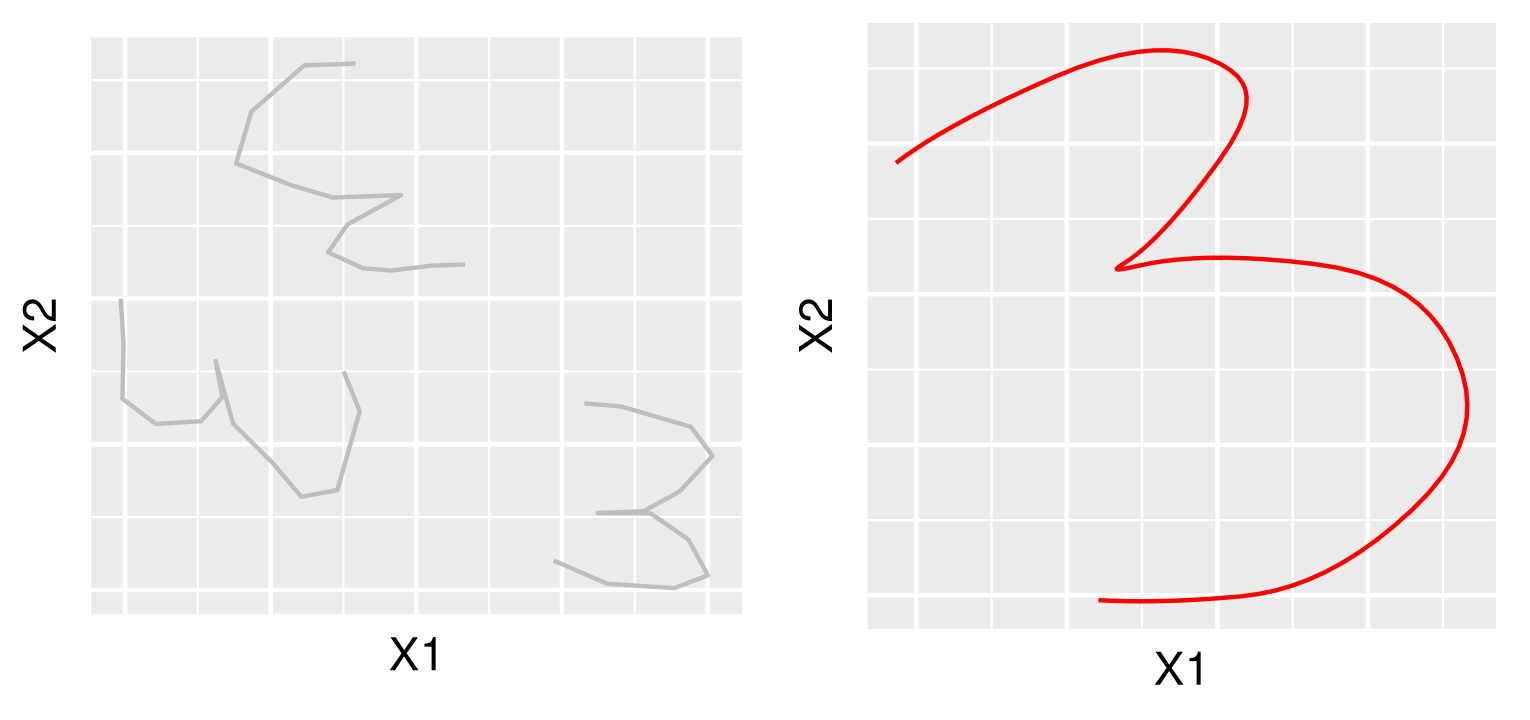
\includegraphics[width=0.95\textwidth]{images/motivation.png}
  \caption{\texttt{digits3.dat} from the \texttt{shapes} package \parencite{shapes} with estimated elastic full Procrustes mean. Data: \textcite{digits3}}
\end{figure}
}


% 0-3
%%%%%%%%%%%%%%%%%%%%%%%%%%%%%%%%%%%%%%%%
%\frame{
%\frametitle{Motivation}
%Calculate \alert{shape means} for \alert{2D curves} observed at discrete points:
%\vspace{-0.5em}
%\begin{columns}
%  \begin{column}{0.48\textwidth}
%    \begin{figure}
%      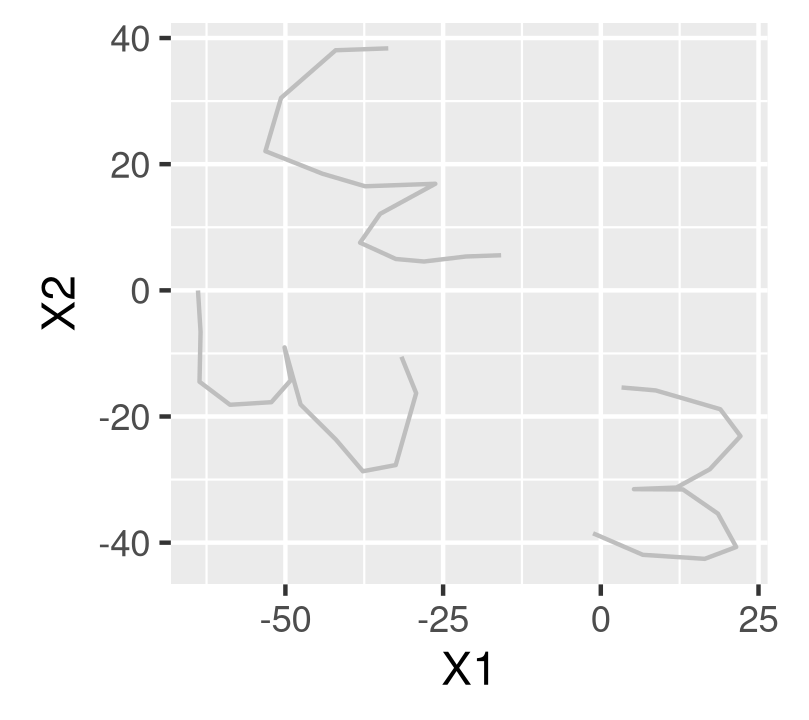
\includegraphics[width=\textwidth]{images/motivation_data.png}
%      \vspace{-2em}
%      \caption{\texttt{digits3.dat} from the \texttt{shapes} package \parencite{shapes}. Data: \textcite{digits3}}
%    \end{figure}
%  \end{column}
%  \begin{column}{0.48\textwidth}
%    \vspace{-5em}
%    \begin{block}{Challenges}
%      \begin{itemize}
%      \item \alert{Sparse} and \alert{irregular} observations
%      \item \alert{Translation}, \alert{scaling}, \alert{rotation}
%      \item \alert{Warping}
%      \end{itemize}
%    \end{block}
%  \end{column}
%\end{columns}
%}



% 0-3
%%%%%%%%%%%%%%%%%%%%%%%%%%%%%%%%%%%%%%%%
\frame{
\frametitle{Outline}
\begin{itemize}
  \item[1.] What is an Elastic Full Procrustes Mean?
  \item[] $\rightarrow$ Sparse and Irregular Planar Curves
  \item[] $\rightarrow$ Elastic Mean and Warping
  \item[] $\rightarrow$ Full Procrustes Mean and Procrustes Fits
  \item[2.] Estimation Strategy
  \item[] $\rightarrow$ Hermitian Covariance Smoothing
  \item[] $\rightarrow$ Estimation of the Procrustes Mean in a Fixed Basis
  \item[] $\rightarrow$ Procrustes Fits
  \item[3.] Results (so far), Problems, Outlook
\end{itemize}
}



%%%%%%%%%%%%%%%%%%%%%%%%%%%%%%%%%%%%%%%%
\section{What is an Elastic Full Procrustes Mean?}
%%%%%%%%%%%%%%%%%%%%%%%%%%%%%%%%%%%%%%%%

% 1-1
%%%%%%%%%%%%%%%%%%%%%%%%%%%%%%%%%%%%%%%%
\frame{
\frametitle{Sparse and Irregular Planar Curves}
How can we compare observations $\beta_i = (\beta_{i1}, \beta_{i2}, \dots, \beta_{im_i})$?
\begin{columns}
  \begin{column}{0.48\textwidth}
    Treat as \alert{functional} data 
    \vspace{-0.3em}
    $$\vspace{-0.3em}\beta_i : [0,1] \rightarrow \mathbb{R}^2$$
    observed on $t_i = (t_{i1}, \dots, t_{im_i})$
    \vspace{-0.3em}
    $$\beta_{i1} = \beta_i(t_{i1}), \dots, \beta_{im} = \beta_i(t_{im_i})$$
    \vspace{-1.3em}
    \begin{block}{Functional Mean}
      \vspace{-1em}
      $$\hat{\mu}(t) = N^{-1}\sum_{i=1}^N \beta_i(t),\, t \in [0,1]$$
    \end{block}
  \end{column}
  \begin{column}{0.48\textwidth}
    \begin{figure}
      \centering
      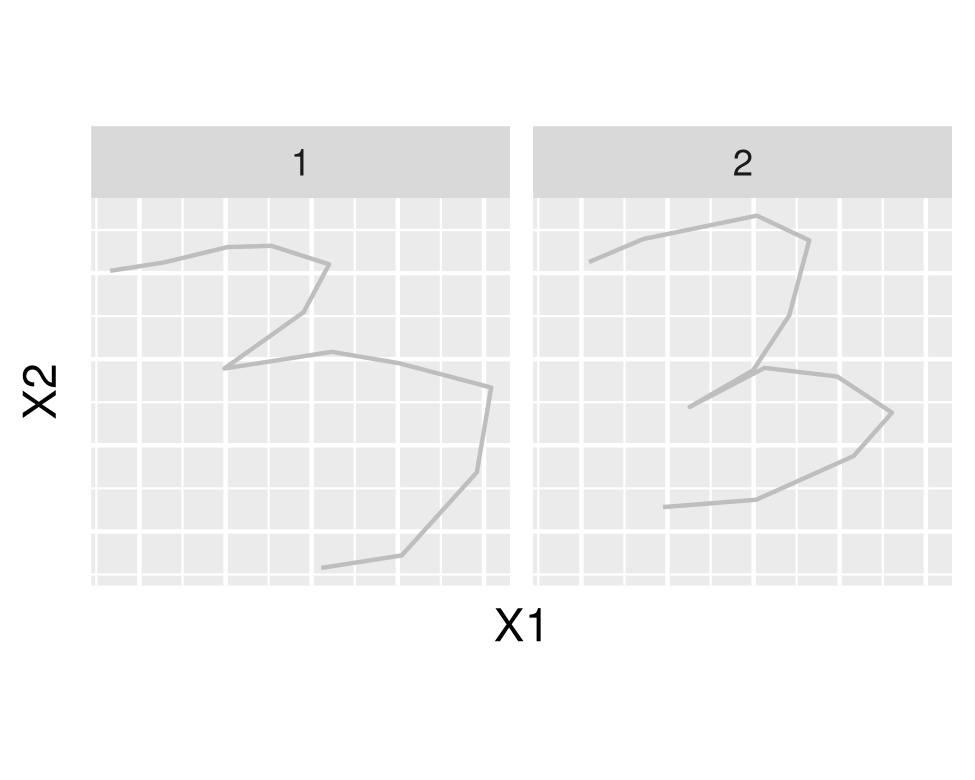
\includegraphics[width=\textwidth]{images/digits3.png}
      \vspace{-2em}
      \caption{\texttt{digits3.dat} from the \texttt{shapes} package \parencite{shapes}. Data: \textcite{digits3}}
    \end{figure}
  \end{column}
\end{columns}
}


% 1-2
%%%%%%%%%%%%%%%%%%%%%%%%%%%%%%%%%%%%%%%%
\frame{
\frametitle{Elastic Mean and Warping}
\begin{itemize}
  \item Parametrisation $t_i = (t_{i1}, \dots, t_{im})$ usually unknown.
    \vspace{0.35em}
  \item Initialize as $t_{ij} = \frac{\text{length of curve i up to point j}}{\text{length of curve i}} \in [0,1]$
\end{itemize}
\vspace{-0.5em}
\begin{columns}
  \begin{column}{0.58\textwidth}
  \begin{figure}
    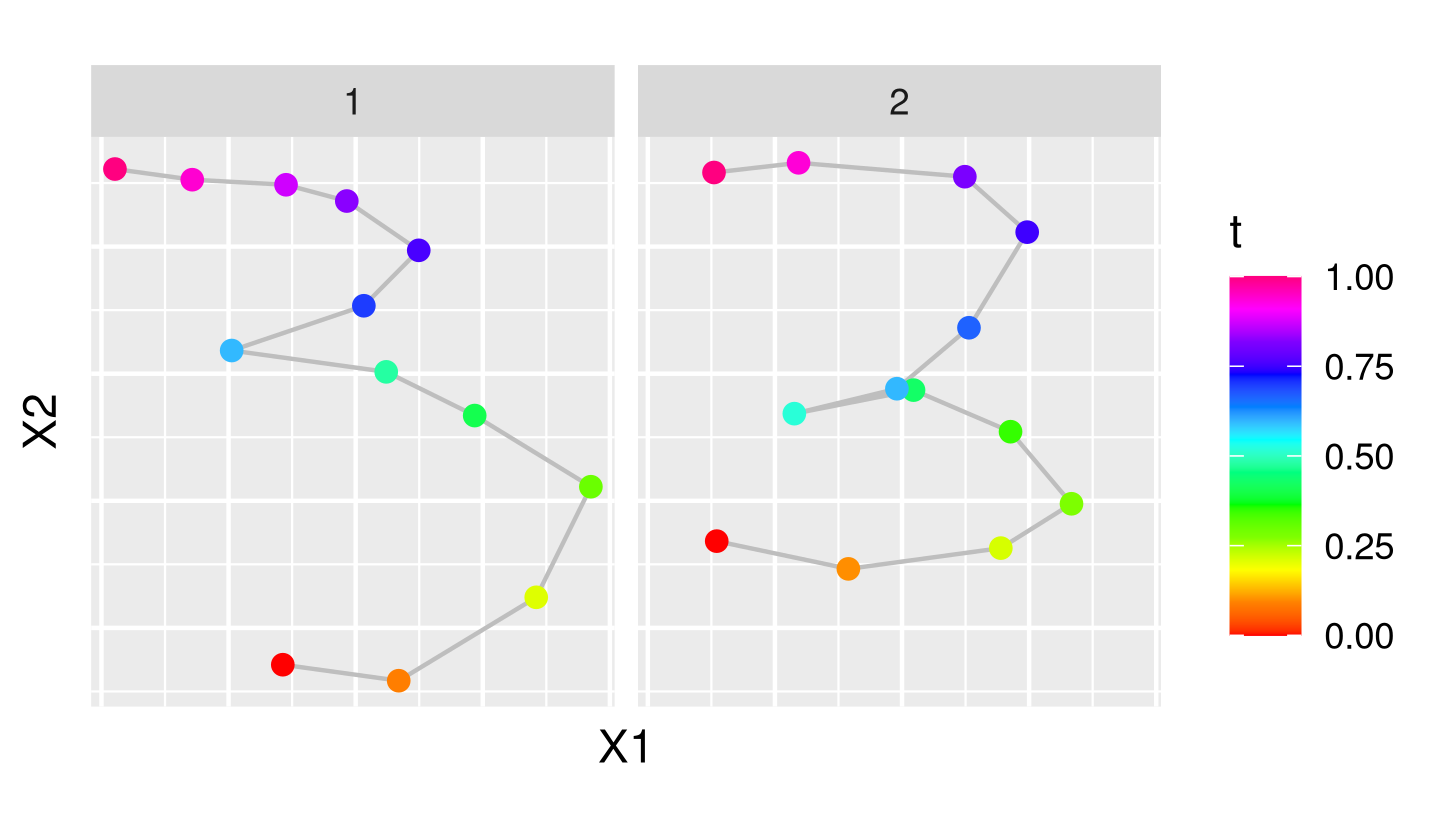
\includegraphics[width=\textwidth]{images/digits3_arcl.png}
    \vspace{-1.3em}
    \caption{with \texttt{get\_arc\_length\_param()} from \texttt{elasdics} \parencite{elasdics}}
  \end{figure}
  \end{column}
  \begin{column}{0.4\textwidth}
    \begin{block}{Functional Mean}
      \vspace{-1em}
      $$\hat{\mu}(t) = N^{-1}\sum_{i=1}^N \beta_i(t)$$
    \end{block}
    \alert{Problem}: $\beta_1(0.5)$, $\beta_2(0.5)$ relate to different \enquote{parts} of the curve
  \end{column}
\end{columns}
}


% 1-3
%%%%%%%%%%%%%%%%%%%%%%%%%%%%%%%%%%%%%%%%
\frame{
\frametitle{Elastic Mean and Warping}
\alert{Problem}: $\beta_1(0.5)$ and $\beta_2(0.5)$ relate to different \enquote{parts} along curve\\
$\rightarrow$ Find a re-parametrization (\alert{warping}) that aligns these parts.
\vspace{-0.3em}
\begin{figure}
  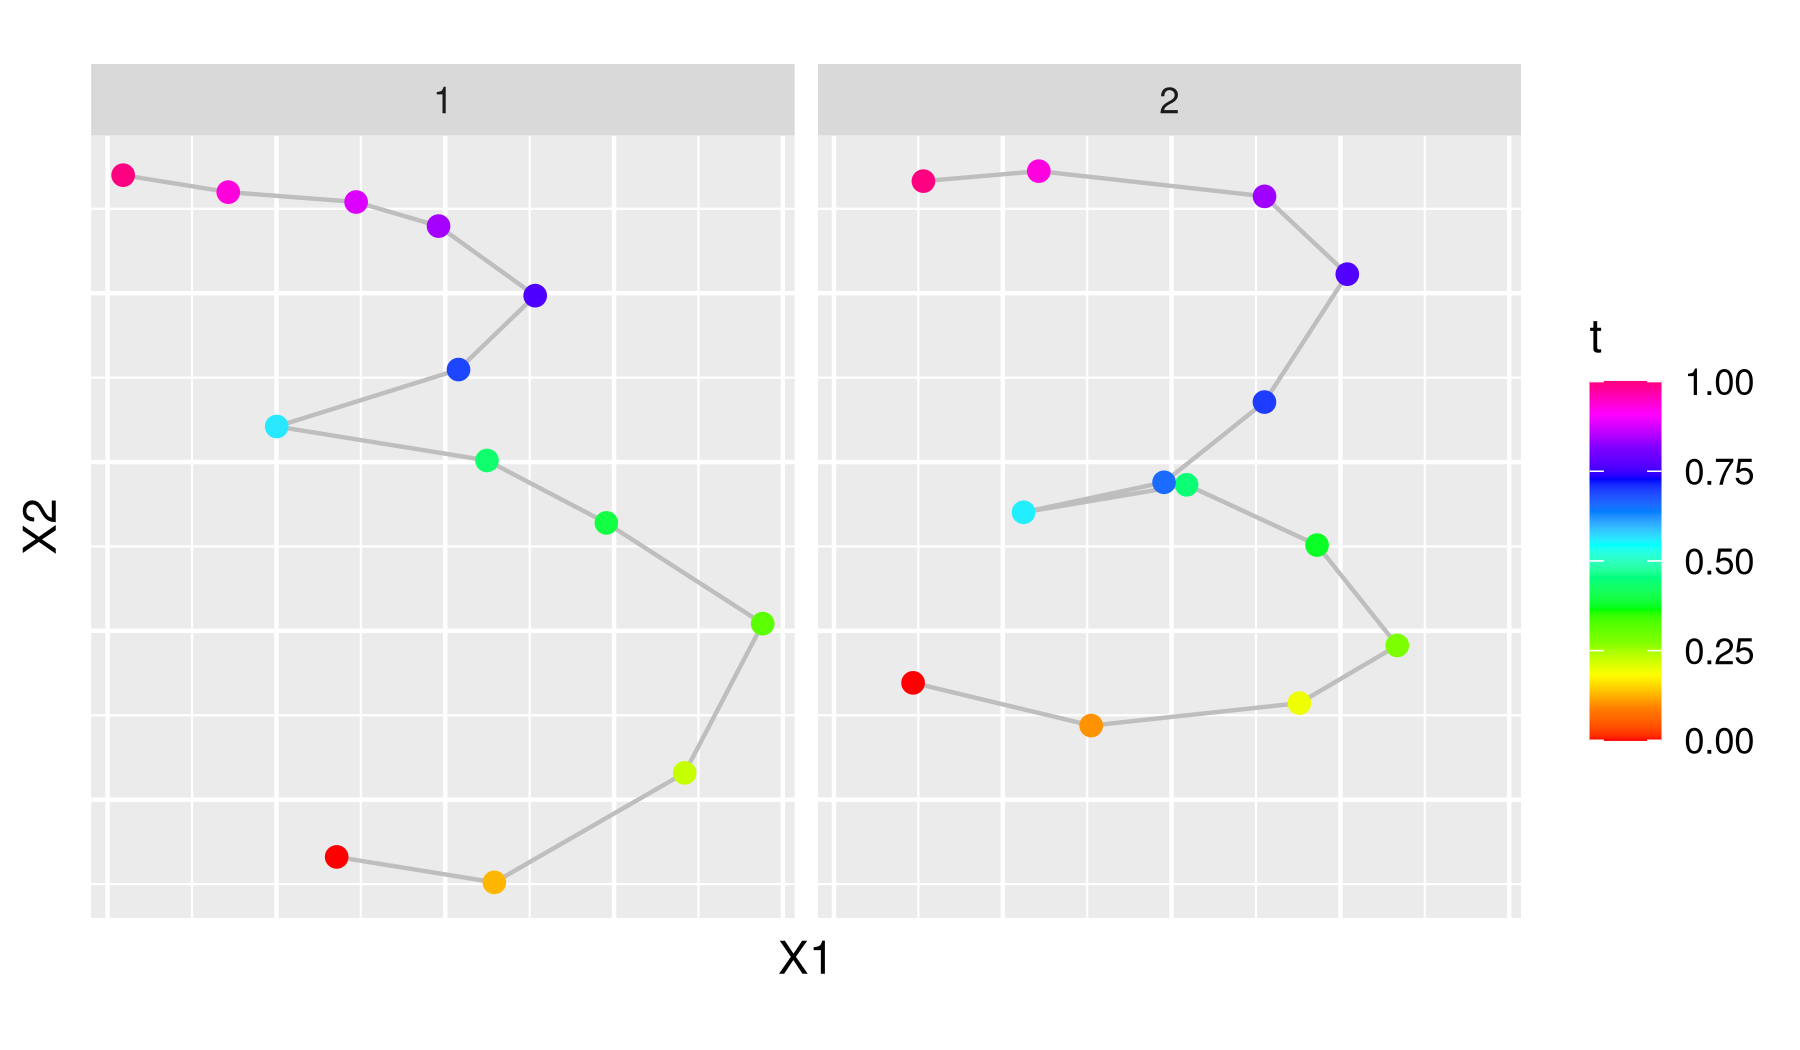
\includegraphics[width=0.7\textwidth]{images/digits3_warp.png}
  \vspace{-1.3em}
  \caption{with \texttt{align\_curves()} from package \texttt{elasdics} \parencite{elasdics}}
\end{figure}
\vspace{-0.3em}
\alert{Note}: Parametrisation relates to speed at which curve is traversed!
}


% 1-4
%%%%%%%%%%%%%%%%%%%%%%%%%%%%%%%%%%%%%%%%
\frame{
\frametitle{Elastic Mean and Warping}
\alert{Note}: Parametrisation relates to speed at which curve is traversed!
\begin{block}{Square-Root-Velocity (SRV) Framework \parencite{Srivasta2011}}
$$ q:[0,1] \rightarrow \mathbb{R}^2, \quad 
  q(t) = \frac{\dot{\beta}(t)}{||\dot{\beta}(t)||} \quad 
  \text{for}\,\,\, ||\dot{\beta}(t)|| \neq 0 $$
\end{block}
\begin{itemize}
  \item Perform \alert{warping alignment} on SRV curves
  \item We can recover original curves $\beta_i$ up to \alert{translation}
  \item Use warping methods for sparse and irregular curves as outlined in \textcite{Steyer2021} and implemented in \texttt{elasdics} \parencite{elasdics}
\end{itemize}
}


% 1-5
%%%%%%%%%%%%%%%%%%%%%%%%%%%%%%%%%%%%%%%%
%\frame{
%\frametitle{Elastic Mean and Warping}
%\alert{Problem}: Methods are not invariant under \alert{scaling} and \alert{rotation}.\\
%\vspace{0.5em}$\rightarrow$ SRV curves have same rotation and $\sqrt{\text{scaling}}$ of data curves.
%\begin{figure}
%  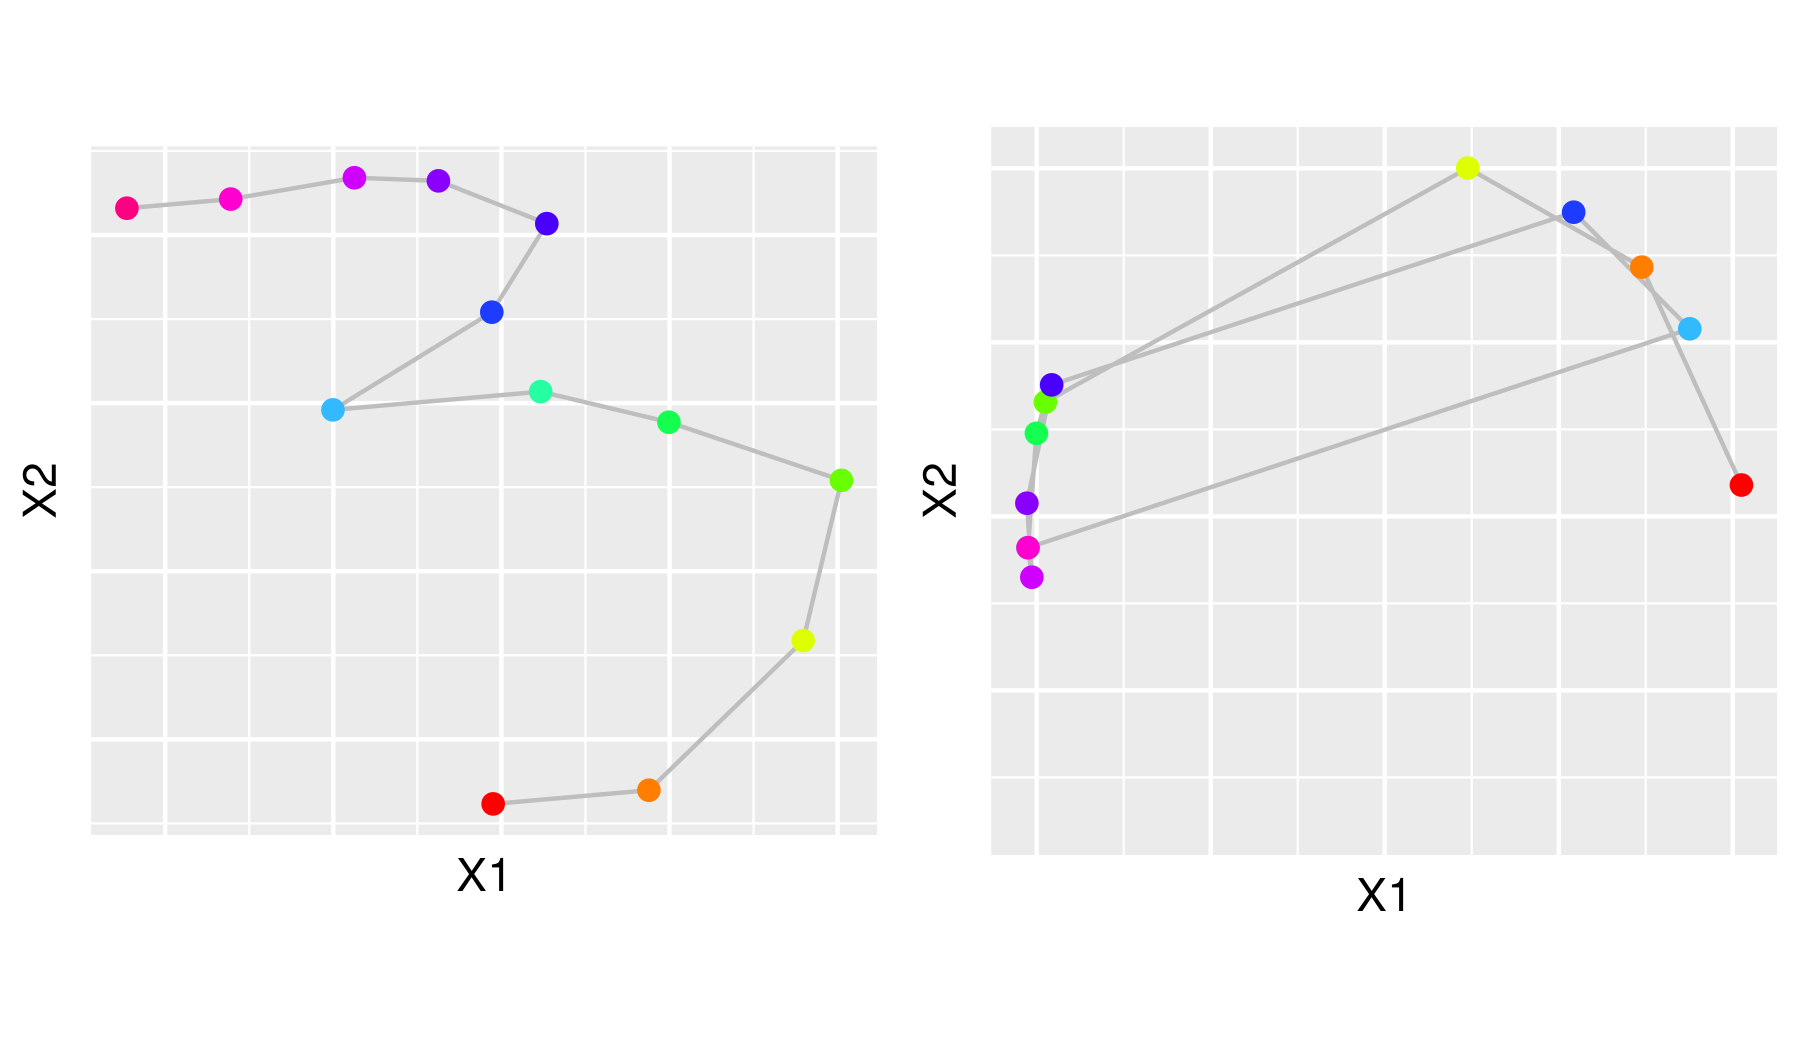
\includegraphics[width=0.7\textwidth]{images/digits3_srv.png}
%  \vspace{-1.3em}
%  \caption{with \texttt{align\_curves()} from package \texttt{elasdics} \parencite{elasdics}}
%\end{figure}
%
%}


% 1-6
%%%%%%%%%%%%%%%%%%%%%%%%%%%%%%%%%%%%%%%%
\frame{
\frametitle{Full Procrustes Mean and Procrustes Fits}
\alert{Problem}: Methods are not invariant under \alert{scaling} and \alert{rotation}.
\\\vspace{0.5em}\textbf{Idea:}
\begin{itemize}
  \item[1.] Calculate SRV \alert{mean} that is invariant under rotation, scaling
  \item[2.] \alert{Align} rotation and scaling of SRV curves to fit the mean
  \item[3.] Perform \alert{warping} on aligned SRV curves
\end{itemize}
\vspace{0.5em}
Well known problem in \textbf{statistical shape analysis} (see e.g. \textcite{DrydenMardia2016}):
\begin{block}{Full Procrustes Distance and Mean}
  $$d_F(q_1, q_2) = \inf_{\Gamma, b} ||q_1 - b \Gamma q_2||$$
  \vspace{-1.5em}
  $$\mu_q : [0,1] \rightarrow \mathbb{R}^2, \quad \hat{\mu}_q = \argmin_{z : [0,1] \rightarrow \mathbb{R}^2} \sum_{i=1}^N d_F(z, q_i)^2$$
\end{block}
}


% 1-7
%%%%%%%%%%%%%%%%%%%%%%%%%%%%%%%%%%%%%%%%
\frame{
\frametitle{Full Procrustes Mean and Procrustes Fits}
Calculation simplifies for \alert{2D shapes} when using \alert{complex} notation:
$$ q_i : [0,1] \rightarrow \mathbb{C}, \quad q_i(t) = x_i(t) + i \, y_i(t) $$
One can show that \parencite[see Ch.\ 8]{DrydenMardia2016}:
\begin{align*}
  \hat{\mu}_q &= \argmin_{z : [0,1] \rightarrow \mathbb{C}} \sum_{i=1}^N 
    \underbrace{1 - \frac{\langle z, q_i \rangle \langle q_i, z \rangle}{\langle z, z \rangle \langle q_i, q_i \rangle}}_{= d_F(z, q_i)^2} \\ 
  &= \argmax_{z : ||z|| = 1} \sum_{i=1}^N \langle z, \tilde{q}_i \rangle \langle \tilde{q}_i, z \rangle, \quad \text{\alert{with}} \quad \tilde{q}_i = \frac{q_i}{||q_i||}\\ 
\end{align*}
\alert{Note}: $\langle q_1, q_2 \rangle = \int_0^1 \overline{q}_1(t) q_2(t) dt, \quad \text{and} \quad ||q_i|| = \sqrt{\langle q_i, q_i \rangle}$
}


% 1-8
%%%%%%%%%%%%%%%%%%%%%%%%%%%%%%%%%%%%%%%%
\frame{
\frametitle{Full Procrustes Mean and Procrustes Fits}
\alert{Note}: $\langle q_1, q_2 \rangle = \int_0^1 \overline{q}_1(t) q_2(t) dt, \quad \text{and} \quad ||q_i|| = \sqrt{\langle q_i, q_i \rangle}$
\vspace{-0.5em}
\begin{align*}
 \hat{\mu}_q  &= \argmax_{z : ||z|| = 1} \sum_{i=1}^N \langle z, \tilde{q}_i \rangle \langle \tilde{q}_i, z \rangle\\ 
  &= \argmax_{z:||z|| = 1} \sum_{i=1}^N \int_0^1 \overline{z}(s) \tilde{q}_i(s) ds \int_0^1 \overline{\tilde{q}}_i(t) z(t) dt \\
  &= \argmax_{z:||z||=1} \int_0^1 \int_0^1 \overline{z}(s) \left( \alert{\sum_{i=1}^N \tilde{q}_i(s) \overline{\tilde{q}}_i(t)} \right) z(t) ds dt
\end{align*}
\vspace{-0.5em}
\begin{itemize}
  \item[$\rightarrow$] sample analouge to $C(s,t) = \mathbb{E}[ \tilde{q}(s) \overline{\tilde{q}}(t)]$ 
  \item[$\rightarrow$] tough to estimate in a sparse setting
\end{itemize}
}


% 1-9
%%%%%%%%%%%%%%%%%%%%%%%%%%%%%%%%%%%%%%%%
\frame{
\frametitle{Full Procrustes Mean and Procrustes Fits}
\textbf{Population level full Procrustes mean:}
$$\mu_q = \argmax_{z:||z|| = 1} \int_0^1 \int_0^1 \overline{z}(s) C(s,t) z(t) ds dt$$
\vspace{-0.5em}
\begin{itemize}
  \item[$\rightarrow$] \alert{Functional PCA} problem (see \textcite{RamsaySilverman2005})
  \item[$\rightarrow$] Solution is the complex leading eigenfunction of $C(s,t)$
  \item[$\rightarrow$] We only need to find a good estimate $\alert{\hat{C}(s,t)}$ to get $\hat{\mu}_q$!
\end{itemize}
\vspace{0.5em}
We can then estimate the rotation and scaling aligned \alert{procrustes fits} as:
$$\hat{q}^P_i = \frac{\langle q_i, \hat{\mu}_q \rangle}{\langle q_i, q_i \rangle} q_i = \langle \tilde{q}_i, \hat{\mu}_q \rangle \tilde{q}_i$$ 
\alert{Note}: For $\vec{x},\vec{y} \in \mathbb{R}^d$:  $\,\cos(\theta) = \frac{\langle \vec{x}, \vec{y} \rangle}{||\vec{x}||\cdot||\vec{y}||} $
}


\section{Estimation Strategy}

% 2-1
%%%%%%%%%%%%%%%%%%%%%%%%%%%%%%%%%%%%%%%%
\frame{
\frametitle{Hermitian Covariance Smoothing}
\alert{Problem}: $\check{C}(s,t) = \frac{1}{N} \sum_{i=1}^N \tilde{q_i}(s) \overline{\tilde{q_i}}(t)$ is not a good estimator \vspace{1em}

Treat estimation of $C(s,t) = \mathbb{E}[ \tilde{q}(s) \overline{\tilde{q}}(t)]$ as a regression problem:
\begin{itemize}
  \item we have observations $y_{ijk} = \tilde{q}_i(t_{ij}) \overline{\tilde{q}}_i(t_{ik})$
  \item treat parametrisation $t_{ij}, t_{ik}$ as \enquote{covariates} $s$ and $t$
  \item non-parametric regression:  $\mathbb{E}[y] = f(s,t)$
  \item use $\hat{C}(s,t) = \hat{f}(s,t)$ for functional PCA
\end{itemize}
\vspace{1em}
\alert{Note}: Difference to $\check{C}(s,t)$:  Smoothing once with all the data vs.\ smoothing $N$ times with little data.
}


% 2-2
%%%%%%%%%%%%%%%%%%%%%%%%%%%%%%%%%%%%%%%%
\frame{
\frametitle{Hermitian Covariance Smoothing}
Using symmetry properties of $C(s,t)$ is important for efficient estimation (see \textcite{Cederbaum2018}).
\vspace{0.5em}

\textbf{Here:} Complex covariance function is \alert{hermitian} $C(s,t) = \overline{C}(t,s)$
$$\mathbb{E}[y] = f_{symm}(s,t) + i \, f_{skew}(s,t)$$
\vspace{-1.2em}
\begin{itemize}
  \item model real and imaginary parts seperately
  \item use \texttt{mgcv} \parencite{Wood2017} with \alert{symmetric} and \alert{skew-symmetric} tensor product P-splines from \texttt{sparseFLMM} \parencite{sparseFLMM}
\end{itemize}
\vspace{0.5em}
\textbf{We get:}
$$\hat{C}(s,t) = b(s)^T \hat{\Xi} b(t), \quad \text{with} \quad \hat{\Xi} = \hat{\Xi}_{symm} + i \, \hat{\Xi}_{skew}$$
}


% 2-2
%%%%%%%%%%%%%%%%%%%%%%%%%%%%%%%%%%%%%%%%
\frame{
\frametitle{Hermitian Covariance Smoothing}
\vspace{-1em}
$$\hat{C}(s,t) = b(s)^T \hat{\Xi} b(t), \quad \text{with} \quad \hat{\Xi} = \hat{\Xi}_{symm} + i \, \hat{\Xi}_{skew}$$
\begin{figure}
  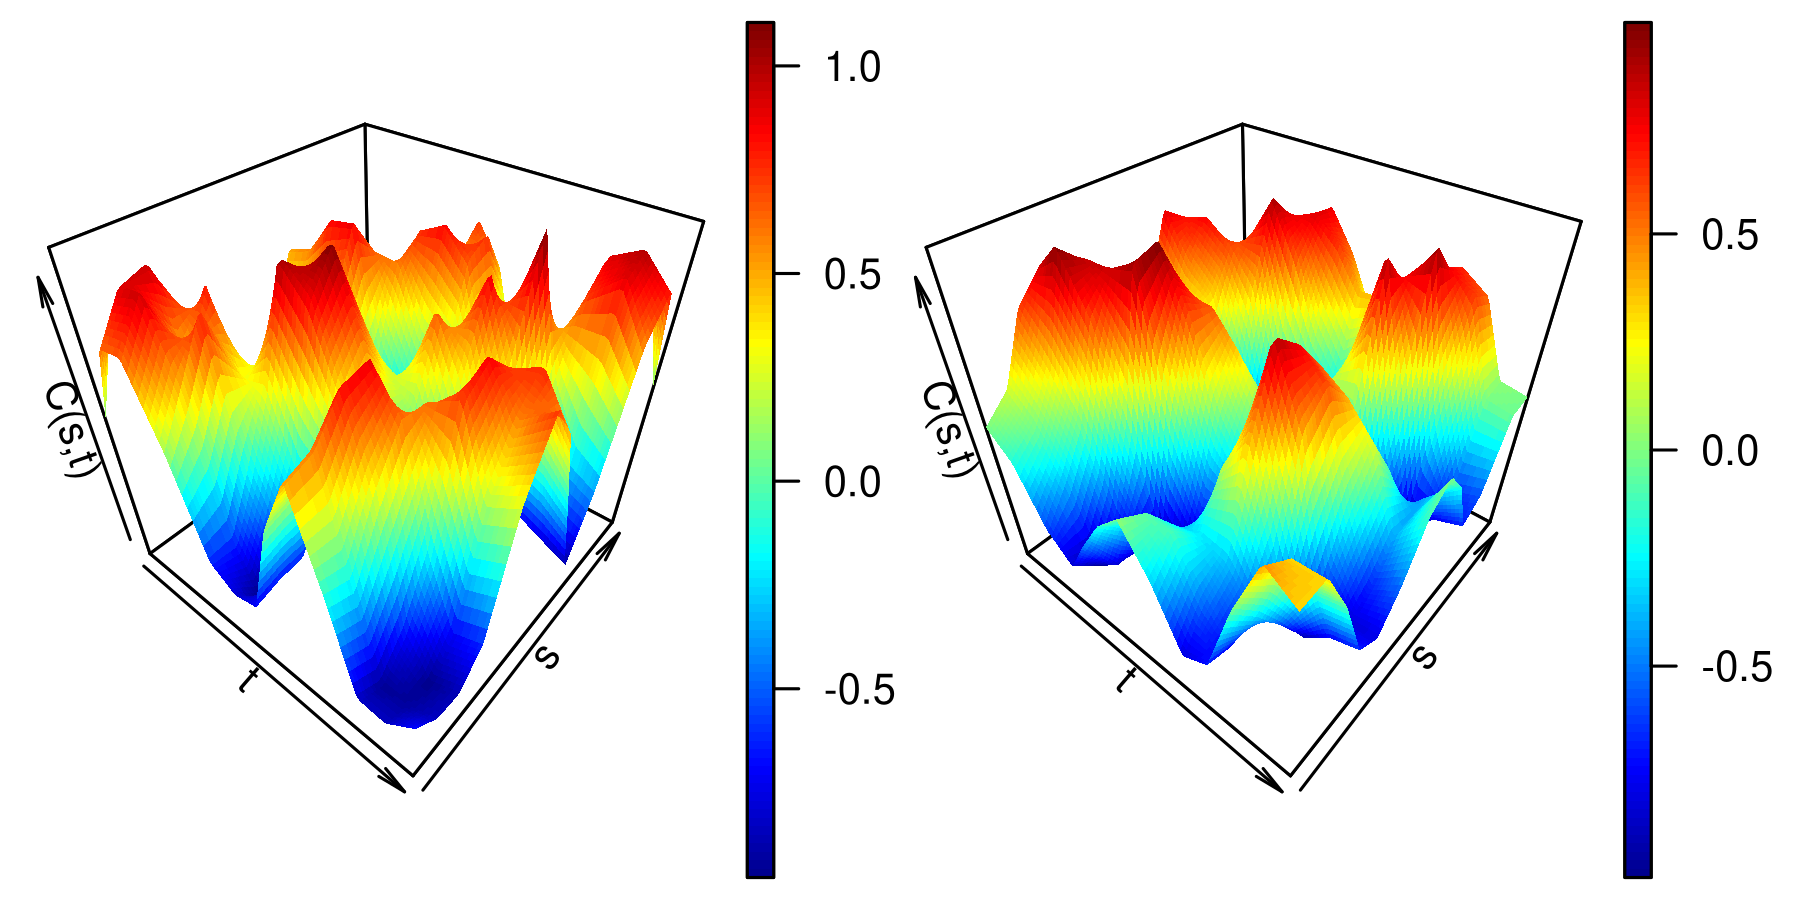
\includegraphics[width=0.75\textwidth]{images/cov_surface_smooth.png}
  \caption{Estimated real (left) and imaginary (right) parts of $C(s,t)$ using P-splines of degree 1, 13 knots and a zero order penalty.}
\end{figure}
\vspace{-0.8em}
$\rightarrow$ How to choose knots, degree and penalty?
}

% 2-3
%%%%%%%%%%%%%%%%%%%%%%%%%%%%%%%%%%%%%%%%
\frame{
\frametitle{Empirical Procrustes Mean in a Fixed Basis}
\textbf{Idea:} Estimate covariance function and mean in the same basis:
$$\hat{\mu}_q(t) = b(t)^T \hat{\theta}_{\mu}, \quad \hat{C}(s,t) = b(s)^T \hat{\Xi} b(t)$$
with real spline basis $b = (b_1, \dots, b_k)$ , $\hat{\theta}_\mu \in \mathbb{C}^k$, $\hat{\Xi} \in \mathbb{C}^{k \times k}$

\vspace{1em}
Then we can solve the optimization problem directly on $\hat{\Xi}$:
$$\hat\theta_\mu = \argmax_{\theta : \theta^H G \theta = 1} \theta^H G \hat{\Xi} G \theta \quad \text{with} \quad G_{kl} = \langle b_k, b_l \rangle $$
$\Rightarrow$ Solution is the leading normalized eigenvector of $\hat{\Xi} G$\\
}


% 2-4
%%%%%%%%%%%%%%%%%%%%%%%%%%%%%%%%%%%%%%%%
\frame{
\frametitle{Procrustes Fits}
Using $\hat{\mu}_q(t) = b(t)^T\hat{\theta}_q$ we can estimate the Procrustes fits:
$$\hat{q}^P_i = \alert{\langle \tilde{q}_i, \hat{\mu}_q \rangle} \tilde{q}_i$$
\vspace{-1.2em}
\begin{itemize}
  \item at the moment: integration with linear interpolation of $\tilde{q}_i$'s
  \item alternative: smoothing in mean basis with $\langle \hat{\tilde{q}}_i, \hat\mu_q \rangle = \hat{\theta}^H_i G \hat{\theta}_\mu$
\end{itemize}
\begin{figure}
  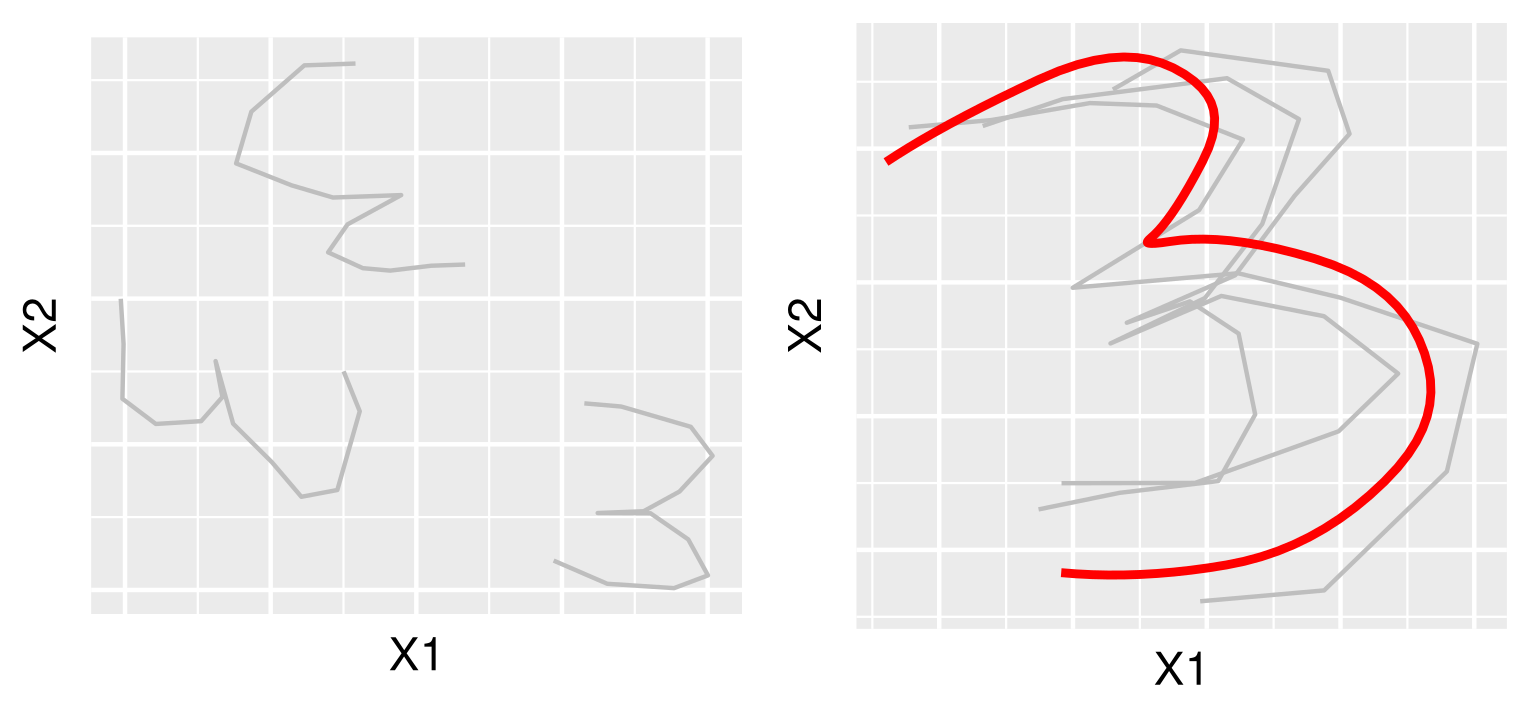
\includegraphics[width=0.75\textwidth]{images/pfit_mean_digits3.png}
  \vspace{-1em}
  \caption{Procrustes fits and mean (on full dataset) before warping.}
\end{figure}
}


\section{Results, Problems, Outlook}
% 3-1
%%%%%%%%%%%%%%%%%%%%%%%%%%%%%%%%%%%%%%%%
\frame{
\frametitle{Results}
\begin{figure}
  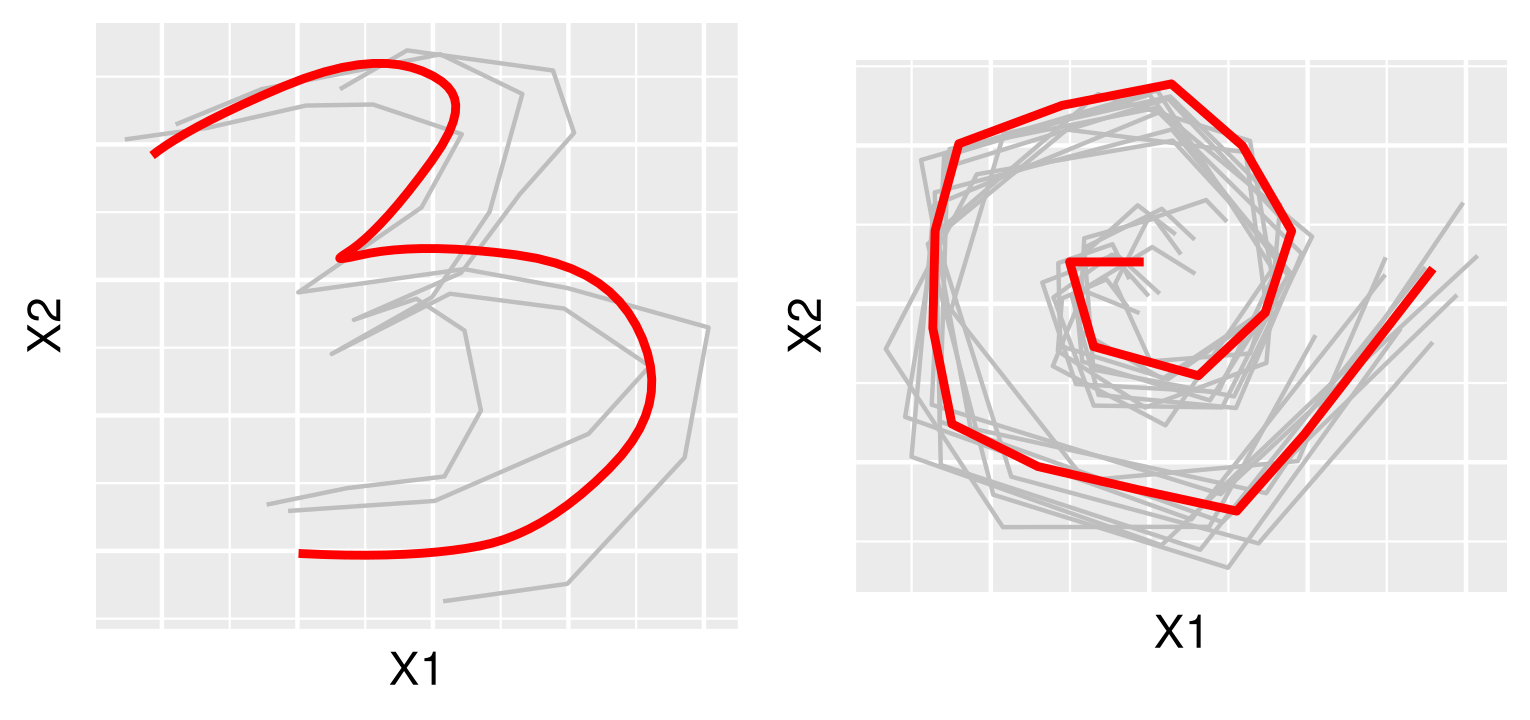
\includegraphics[width=0.75\textwidth]{images/results_digits3_spirals.png}
  \vspace{-1em}
  \caption{Elastic full Procrustes mean and procrustes fits for piecewise linear (left) and piecewise constant (right) splines on SRV level.}
\end{figure}
\begin{itemize}
  \item[$\rightarrow$] Consistent results for piecewise constant splines and zero order penalty.
\end{itemize}
}


% 3-2
%%%%%%%%%%%%%%%%%%%%%%%%%%%%%%%%%%%%%%%%
\frame{
\frametitle{Problems}
\textbf{Normalization:} $\tilde{q}_i = \frac{q_i}{||q_i||}$ is itself an estimate ($||q_i|| = \sqrt{\alert{\langle q_i, q_i \rangle}}$)
\begin{itemize}
  \item[$\rightarrow$] can either restrict $\beta_i$'s to unit--length or normalize $q_i$ directly
  \item[$\rightarrow$] likely need smoothing (in the mean basis?) for this
\end{itemize}
\vspace{-0.3em}
\begin{figure}
  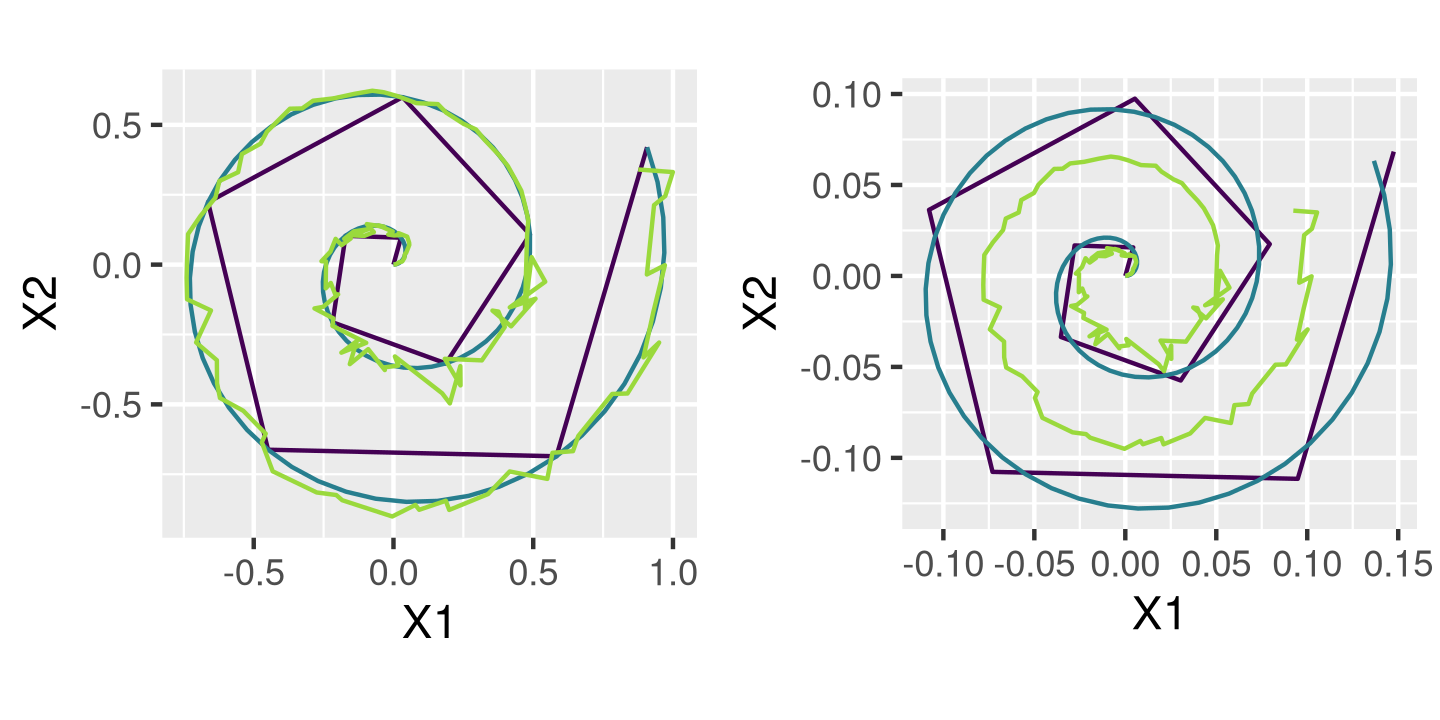
\includegraphics[width=0.7\textwidth]{images/normalization.png}
  \vspace{-1.3em}
  \caption{Spirals (left) and unit--length spirals (right).}
\end{figure}
\vspace{-0.5em}
$\rightarrow$ only ok, as long as all curves have same "amount" of sparsity 
}


% 3-3
%%%%%%%%%%%%%%%%%%%%%%%%%%%%%%%%%%%%%%%%
\frame{
\frametitle{Outlook}
\textbf{ToDo:}
\begin{itemize}
  \item Better normalization / estimation of procrustes fits
  \item Real world data application (open curves)
  \item Mean for closed curves
  \item Real world data application (closed curves)
\end{itemize}
\vspace{1em}
\textbf{Nice to have (maybe later):}
\begin{itemize}
  \item Cover codebase with testcases (make it *really* solid)
  \item Disentangle codebase from \texttt{elasdics} and package it
  \item Reduce bloat / make it faster
\end{itemize}
\vspace{1em}
\textbf{Timeline:} Would like to be finished by July 
}

% Appendix
%%%%%%%%%%%%%%%%%%%%%%%%%%%%%%%%%%%%%%%
\section{Appendix}
\nocite{*}
\frame[allowframebreaks]{
\printbibliography
}




\end{document}
